\documentclass[a4paper,12pt,twoside]{article}
\usepackage[polish]{babel}

\addto\captionspolish{\renewcommand{\figurename}{Rys.}}
\usepackage[utf8]{inputenc}
\usepackage[english]{babel}
\usepackage[margin=2cm]{geometry}
\usepackage[table,xcdraw]{xcolor}
\usepackage{graphicx}
\usepackage{indentfirst}
\usepackage{multicol}
\usepackage{listings}
\usepackage[T1]{fontenc}
\usepackage{bigfoot} % to allow verbatim in footnote
\usepackage[numbered,framed]{matlab-prettifier}
\usepackage{filecontents}
\usepackage{blindtext}
\usepackage{graphics}
\usepackage{adjustbox}
\usepackage{float}
\usepackage{subfigure}
\usepackage{multirow}
\usepackage{colortbl}
\usepackage{anyfontsize}
\usepackage{t1enc}
\usepackage{enumitem}
\usepackage{hhline}
\usepackage{fancyhdr}
\usepackage{marginnote}
\usepackage{amsmath}
\usepackage{amsthm}
\usepackage{mathtools}
\usepackage{dirtytalk}
\usepackage{cite}
\usepackage[font=footnotesize, labelfont=bf]{caption}
\usepackage{textgreek} %for units like micro in text
\usepackage[hidelinks]{hyperref}
\usepackage{adjustbox}
\urlstyle{same}
\usepackage{physics}
\usepackage{chemfig}
\renewcommand{\figurename}{Rys.}
\title{\textbf{Projekt 3: Generatory liczb pseudolosowych: rozkłady skorelowane w 2D.}}
\author{Kacper Połuszejko, 412183}
\date{}
\begin{document}
\maketitle

\section*{Wstęp}

Celem ćwiczenia było wygenerowanie rozkładów dwuwymiarowych: normalnego, jednorodnego w kole 2D, oraz transformację afiniczną (koło --> elipsa), a także wyznaczenie macierzy kowariancji (dla tej ostatniej).

 \section{Metodyka}

 \subsection{Rozkład sferycznie konturowany - normalny}

 Stosujemy metodę Boxa-Mullera:

 
\begin{equation}
    \begin{gathered}
        U_1 \sim U(0,1), \quad U_2 \sim U(0,1) \\
        X = \sqrt{-2 \ln(1 - U_1)} \cos(2\pi U_2), \quad X \sim N(0,1) \\
        Y = \sqrt{-2 \ln(1 - U_1)} \sin(2\pi U_2), \quad Y \sim N(0,1)
    \end{gathered} \tag{1} \label{eq:1}
\end{equation}

 Wektory $(X,Y)$ mają rozkład sferycznie konturowany, ponieważ ich gęstość zależy tylko od odległości od środka rozkładu.

 \subsection{Rozkład jednorodny w kole}

 Na podstawie rozkładu sferycznie konturowanego można umieścić wygenerowane punkty na obwodzie okręgu o promieniu jednostkowym, normalizując zmienne:

\begin{equation}
    \begin{gathered}
    X' = \frac{X}{\sqrt{X^2 + Y^2}} \\
    Y' = \frac{Y}{\sqrt{X^2 + Y^2}}
    \end{gathered} \tag{2} \label{eq:2}
\end{equation}


 Następnie można przesunąć je do środka okręgu, skalując zmienne w następujący sposób:

 \begin{equation}
    \begin{gathered}
    X'' = RX' \\
    Y'' = RY' \\
    R = \sqrt{U1}, \quad U1 \sim U(0,1)
    \end{gathered} \tag{3} \label{eq:3}
\end{equation}

Wektory $(X'', Y'')$ mają rozkład jednorodny w kole o promieniu jednostkowym.

\subsection{Transformacja afiniczna: koło $\rightarrow$ elipsa}

Rozkład dwuwymiarowy możemy podać transformacji liniowej (afinicznej), która przekształci koło w elipsę. Docelowy kształt elipsy definiujemy, podając macierz transformacji $A = [\vec{r_1}, \vec{r_2}]$, gdzie $\vec{r_1}$ i $\vec{r_2}$ to wektory określające półosie główne. \\
Macierz A określa więc obrót oraz skalowanie wzdłuż półosi głównych. \\

 Ponieważ półosie główne elipsy muszą być ortogonalne, tak jak wersory układu kartezjańskiego, wystarczy więc tylko obrócić je o zadany kąt $\alpha$ przy użyciu macierzy obrotu $R_{\alpha}$ i przeskalować ich długości:


\begin{equation}
    \begin{gathered}
        \vec{r}_1 = b_1 R_{\alpha} \hat{e}_x, \quad \hat{e}_x = \begin{bmatrix} 1 \\ 0 \end{bmatrix}^T \\
        \vec{r}_2 = b_2 R_{\alpha} \hat{e}_y, \quad \hat{e}_y = \begin{bmatrix} 0 \\ 1 \end{bmatrix}^T \\
        R_{\alpha} =
        \begin{bmatrix}
            \cos(\alpha) & -\sin(\alpha) \\
            \sin(\alpha) & \cos(\alpha)
        \end{bmatrix}, \quad \alpha \in [0, 2\pi]
    \end{gathered} \tag{4} \label{eq:4}
\end{equation}

gdzie $b_1$ i $b_2$ to współczynniki skalujące. \\

\subsection{Macierz kowariancji}

Macierz kowariancji ma postać:

\begin{equation}
    \begin{gathered}
        \Sigma =
        \begin{bmatrix}
            \sigma_x^2 & \sigma_{xy} \\
            \sigma_{yx} & \sigma_y^2
        \end{bmatrix},
        \quad \quad
        \sigma_{xy} = \sigma_{yx},
    \end{gathered} \tag{5}
\end{equation}

jej elementy możemy wykorzystać do wyznaczenia współczynnika korelacji:

\begin{equation}
r_{xy} = \frac{\sigma_{xy}}{\sqrt{\sigma_x^2 \sigma_y^2}}. \tag{6}
\end{equation}


Macierz kowariancji można wyznaczyć ze wzoru:
\[
\Sigma = A D A^T,
\]
gdzie A jest macierzą transformacji. \\
Dla pierwotnego rozkładu \( N^2(0,1) \) macierz $D$ jest postaci:
\[
D =
\begin{bmatrix}
    \sigma_x^2 & 0 \\
    0 & \sigma_y^2
\end{bmatrix}
=
\begin{bmatrix}
    1 & 0 \\
    0 & 1
\end{bmatrix} = I
\]
w związku z tym $\Sigma$ ma prostą konstrukcję
\[
\Sigma = A A^T \quad \rightarrow \quad \Sigma^{-1} = (A^T)^{-1} A^{-1}
\]
Jeśli oznaczymy
\[
A^{-1} \vec{r}' = \vec{z}
\]
to losując wektory \( \vec{z} \) z rozkładu \( N^2(0,1) \) dostaniemy rozkład skorelowany
\[
\vec{r}' = A \vec{z}
\]
określony macierzą kowariancji \( \Sigma = A A^T \)


 
\section{Wyniki}

\subsection{Rozkład sferycznie konturowany - normalny}

Wylosowano $n = 10^4$ punktów z dwuwymiarowego rozkładu normalnego $N^2(0,1)$ przy użyciu metody Boxa-Mullera. 
 
 \begin{figure}[h!]
    \centering
        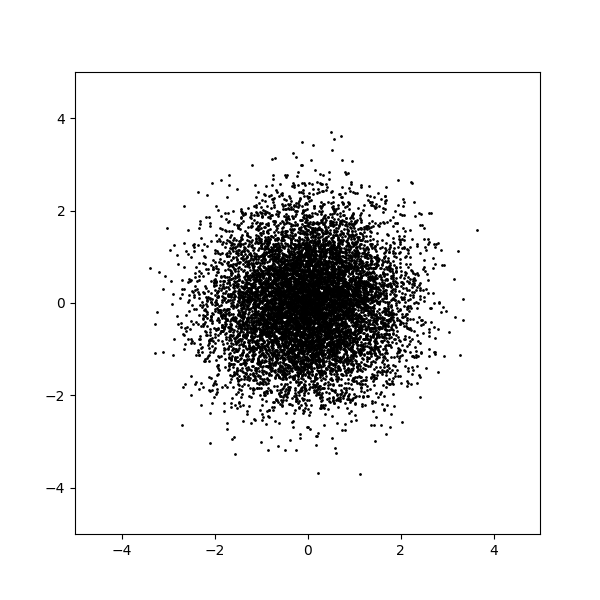
\includegraphics[scale = 0.6]{Carlo_1.png}
    \caption{Rozkład normalny w 2D wygenerowany za pomocą metody Boza-Mullera (\ref{eq:1}) }
\end{figure}

 \subsection{Rozkład jednorodny w kole}

Za pomocą wzorów (\ref{eq:2}) oraz (\ref{eq:3}) wygenerowano rozkład jednorodny na okręgu oraz w kole. 

 \begin{figure}[h!]
    \begin{minipage}{0.55\textwidth}
        \centering
        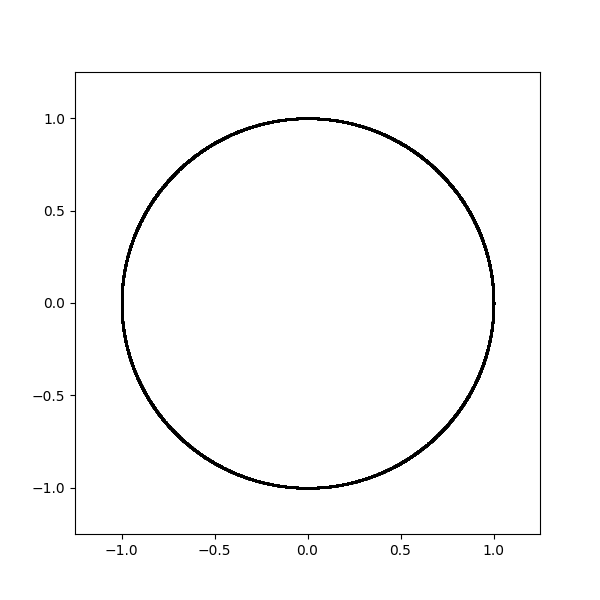
\includegraphics[scale = 0.5]{Carlo_2.png}
    \end{minipage}
    %\hspace{15mm}
    \begin{minipage}{0.55\textwidth}
        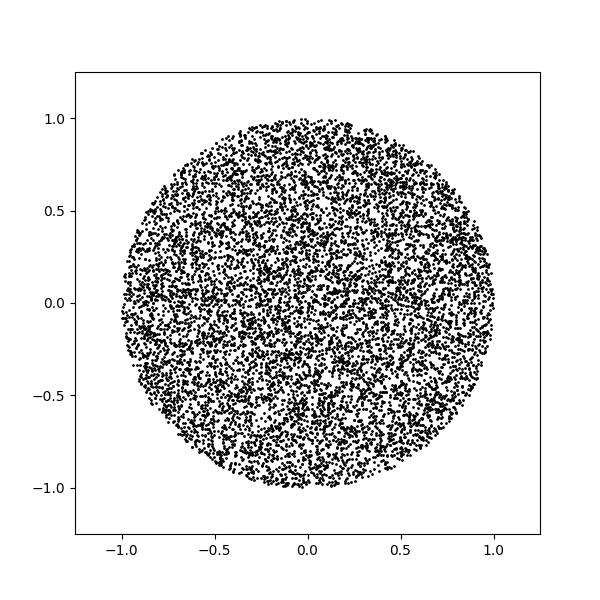
\includegraphics[scale = 0.5]{Carlo_3.png}
    \end{minipage}
    \caption{Rozkład jednorodny na okręgu (po lewej) oraz w kole (po prawej).  }
\end{figure}

\subsection{Transformacja afiniczna}

Za pomocą wzorów \ref{eq:4} dokonano transformacji dwóch rozkładów: normalnego w 2D (\textbf{Rys. 1}) oraz jednorodnego w kole (\textbf{Rys. 2}). Przyjęte parametry: $\alpha = \frac{\pi}{4}$, $b_1 = 1$, $b_2 = 0.2$ . \\

Macierz transformacji $A$ wyniosła więc:

\begin{equation*}
A = 
    \begin{bmatrix}
            0.71 & -0.14 \\
            0.71 & 0.14
    \end{bmatrix}.
\end{equation*}


 \begin{figure}[h!]
    \begin{minipage}{0.55\textwidth}
        \centering
        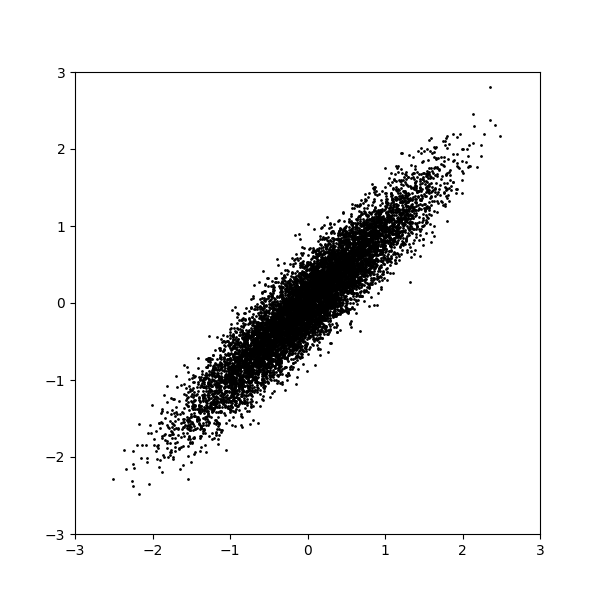
\includegraphics[scale = 0.5]{Carlo_5.png}
    \end{minipage}
    %\hspace{15mm}
    \begin{minipage}{0.55\textwidth}
        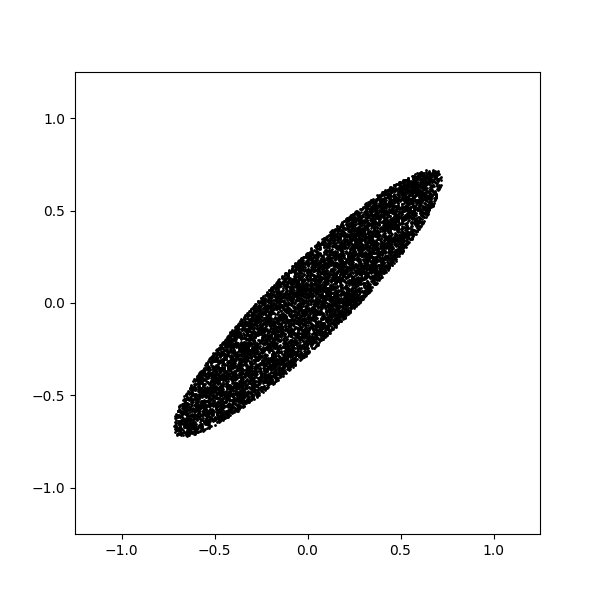
\includegraphics[scale = 0.5]{Carlo_4.png}
    \end{minipage}
    \caption{Przetransformowany rozkład normalny $N^2(0,1)$ (po lewej) oraz rozkład skorelowany w elipsie (po prawej).  }
\end{figure}

\subsection{Macierz kowariancji oraz współczynnik korelacji}

\subsubsection{Rozkład skorelowany w elipsie}
Macierz kowariancji wyniosła:

\begin{equation*}
    \Sigma \simeq
    \begin{bmatrix}
            0.13 & 0.12 \\
            0.12 & 0.13
    \end{bmatrix}.
\end{equation*}

Współczynnik korelacji: $r_{xy} \simeq 0.92$.

\subsubsection{Skorelowany rozkład gaussa}

Macierz kowariancji wyniosła:

\begin{equation*}
    \Sigma \simeq
    \begin{bmatrix}
            0.52 & 0.48 \\
            0.48 & 0.53
    \end{bmatrix}.
\end{equation*}
Co jest w przybliżeniu równe teoretycznemu wyrażeniu $\Sigma = AA^T$ .

Współczynnik korelacji: $r_{xy} \simeq 0.92$.


\end{document}
